\section{Universality and the curvature coupling}\label{rep:h-universality}

The threshold $\lamc\approx-0.01$ does not depend on the details of one point in parameter space, and its use as a survival criterion requires a condition on the Higgs curvature coupling.
We show that the duration of the turn enters only logarithmically, that the couplings enter with logarithmic derivatives below $0.7$, and that sectors with 't~Hooft flux cannot turn around. %
A finite threshold exists in every sector that can host a turning point and keeps a Higgs zero mode, because there the zero-point motion of the constant gauge modes still confines the zero mode, so that for $\lambda<0$ it is a resonance and a finite duration gives a finite threshold (Sec.~\ref{sec:rb-spin}); we compute $\lamc\approx-0.01$ for the AAA structure, and an indicative estimate gives a threshold of the same size for the PPA and PAA structures. %
For the curvature coupling we find that the survival probability stays within $1\%$ of its conformal value for $\xiH(\mub)\gtrsim\xiHcentral$ at the measured top mass, or $\gtrsim\xiHmin$ including all prescription variants ($\approx\xiHminEW$ at the electroweak scale), and for $\xiH(\mub)\gtrsim\xiHhalf$ at the point $\Pone=1/2$. %
This zero-mode condition is stronger than the all-mode bound from the subsequent inflation for $m_t\gtrsim172.1\GeV$, and the conformal value $\xiH=1/6$ satisfies both. %

\subsection{Duration of the turn}
\label{sec:rb-duration}

Changing only the duration of the turn at fixed $\Lb$ (that is, changing $h$) leaves $\mub$ and every node coupling unchanged, so $\Gamma(\tau)$ is unchanged and $\eta_\infty\to f\eta_\infty$ is exactly equivalent to $I\to fI$ in Eq.~(\ref{eq:rb-hazard}).
Near threshold the width has the WKB form of Sec.~\ref{sec:rb-size}, $I\simeq A_{\rm eff}\eta_\infty\exp(-b_{\rm eff}|\lambda|^{-1/2})$ with $\lambda\equiv\lambda(\mub)$.
Holding $I$ fixed at the value that defines a level of $\Pone$, $\ln\eta-b_{\rm eff}|\lamc|^{-1/2}$ is constant, so
\begin{align}
|\lamc(\eta)|^{-1/2}&=|\lamc(\eta_0)|^{-1/2}+\frac{\ln(\eta/\eta_0)}{b_{\rm eff}},\nonumber\\
\frac{d\lamc}{d\ln\eta_\infty}&=\frac{2|\lamc|^{3/2}}{b_{\rm eff}},\qquad
\frac{dm_c}{d\ln\eta_\infty}=-\frac{2|\lamc|^{3/2}}{b_{\rm eff}\,|d\lambda(\mub)/dm_t|},
\label{eq:rb-eta}
\end{align}
where the last relation uses $\lamc\equiv\lambda_{\rm SM}(\mub;m_c)$ and Eq.~(\ref{eq:rb-lin}).
With $b_{\rm eff}=1.40$, $1.30$, and $1.19$ this gives $dm_c/d\ln\eta_\infty=-0.19$, $-0.31$, and $-0.47\GeV$ at $\Pone=0.9$, $0.5$, and $0.1$; equivalently $|\lamc|\propto\eta_\infty^{-0.137}$, $\eta_\infty^{-0.170}$, and $\eta_\infty^{-0.208}$. %

\begin{table}[t]
\centering
\caption{Hazard-equivalent threshold $\lamc(\mub)$ when the conformal duration is changed to $f\eta_\infty$ at fixed node widths (earlier model).
The entries for $f=0.25$, $\Pone=0.1$ and $f=4$, $\Pone=0.9$ use a linear extrapolation of $\ln I$ beyond the mass grid by at most $0.2\GeV$.} %
\label{tab:rb-eta}
\begin{tabular}{cccc}
\toprule
$f$ & $\Pone=0.9$ & $\Pone=0.5$ & $\Pone=0.1$ \\
\midrule
$0.25$ & $-0.011156$ & $-0.015745$ & $-0.020655$ \\ %
$0.5$ & $-0.010039$ & $-0.013698$ & $-0.017672$ \\ %
$1$ & $-0.009104$ & $-0.012104$ & $-0.015140$ \\ %
$2$ & $-0.008306$ & $-0.010820$ & $-0.013233$ \\ %
$4$ & $-0.007618$ & $-0.009759$ & $-0.011734$ \\ %
\bottomrule
\end{tabular}
\end{table}

Table~\ref{tab:rb-eta} gives the direct recalculation.
Equation~(\ref{eq:rb-eta}) agrees with it to $0.6\%$ when $\eta_\infty$ changes by a factor of 2 and to $1.3\%$ for a factor of 4; its only error is the $\lambda$ dependence of the local exponent, a second-order effect. %
Halving or doubling the duration moves $m_c$ by $+0.24$ or $-0.20\GeV$ at $\Pone=1/2$ ($+0.14/-0.12$ and $+0.38/-0.29\GeV$ at $\Pone=0.9$ and $0.1$). %
An independent full-chain recalculation with $h\Lb$ changed by $e^{\pm1}$, in which $\mub$ and the node couplings move as well, agrees with Eq.~(\ref{eq:rb-eta}) to $1$--$3\%$ (Sec.~\ref{sec:rb-background}). %
The magnitude of $\lamc$ follows from Eq.~(\ref{eq:rb-lamc-size}): doubling or halving $\eta_\infty$ changes $|\lamc|$ by $-11\%$ or $+13\%$. %

\subsection{Dependence on the couplings}
\label{sec:rb-couplings}

We multiply the node couplings by $1\pm0.1$ at fixed $\lambda(\mu)$, one coupling at a time, recompute the Gaussian profiles, the matching, the cross terms, and the two-dimensional roots at five nodes and five masses, and convert the width ratios into hazards.
This study uses the earlier model; for unit multipliers the variant code reproduces its roots to $5\times10^{-12}$ in $\Gamma$, and the $+10\%$ and $-10\%$ sides are symmetric to within $5\%$. %
At $\Pone=1/2$ we find
\begin{equation}
\frac{\partial\ln|\lamc|}{\partial\ln g_2}=0.66,\qquad \frac{\partial\ln|\lamc|}{\partial\ln g_Y}=0.16,\qquad \frac{\partial\ln|\lamc|}{\partial\ln y_t}=0.63, %
\label{eq:rb-coupderiv}
\end{equation}
nearly the same at $0.9$ and $0.1$ for $g_2$ and $g_Y$, and within $10\%$ for $y_t$ ($0.575$, $0.627$, $0.649$). %
Increasing any of the three couplings makes $\lamc$ more negative and the zero mode more stable.
Locally,
\begin{equation}
|\lamc|\approx0.0121\Bigl(\frac{\eta_\infty}{300}\Bigr)^{-0.17}\Bigl(\frac{g_2}{0.528}\Bigr)^{0.66}\Bigl(\frac{g_Y}{0.443}\Bigr)^{0.16}\Bigl(\frac{y_t}{0.430}\Bigr)^{0.63}, %
\label{eq:rb-powerlaw}
\end{equation}
with the couplings taken at the first node; larger changes should use the logarithmic form of Eq.~(\ref{eq:rb-eta}).

\paragraph{WKB decomposition.}
The same structure explains these exponents.
Write the hazard as $I=A\,e^{-b|\lambda|^{-1/2}}$, where $A$ and $b$ depend on a coupling $g_i$.
The sensitivity at fixed $\lambda$ is then $s_i\equiv\partial\ln I/\partial\ln g_i=\alpha_i-\beta_i|\lambda|^{-1/2}$, with $\alpha_i=\partial\ln A/\partial\ln g_i$ and $\beta_i=\partial b/\partial\ln g_i$.
Holding $I$ fixed then gives
\begin{equation}
\frac{\partial\ln|\lamc|}{\partial\ln g_i}=2\,\frac{\partial\ln b}{\partial\ln g_i}-\frac{2\alpha_i}{S_c},\qquad S_c=\frac{b_{\rm eff}}{|\lamc|^{1/2}}=14.7,\ 11.8,\ 9.7 . %
\label{eq:rb-wkb-decomp}
\end{equation}
Fits of the measured $s_i$ predict $0.685$, $0.666$, and $0.658$ for $g_2$, $0.173$, $0.166$, and $0.161$ for $g_Y$, and $0.527$, $0.597$, and $0.681$ for $y_t$ at the three levels, within $3\%$ ($g_2$, $g_Y$) and $8\%$ ($y_t$) of the direct values; the exponent $b$ itself scales as $g_2^{0.60}g_Y^{0.16}y_t^{0.19}$ at $\Pone=1/2$. %

\paragraph{Zero-point scaling does not explain the threshold.}
A pure zero-mode scaling, $H=g^{2/3}h(\lambda/g^2)$, would give $\Gamma=g^{2/3}F(\lambda/g^2)$, so $b\propto g$ and $A\propto g^{2/3}$, and by Eq.~(\ref{eq:rb-wkb-decomp}) a common gauge exponent $2-4/(3S_c)=1.89$; the computed exponent is $0.83$. %
A direct test confirms this: multiplying $g_2$ and $g_Y$ by $1.1$ and $\lambda$ by $1.21$, so that $\lambda/g^2$ is fixed, should multiply $\Gamma$ by $1.1^{2/3}=1.066$, but the computed ratio at $\tau=0$ is $2.54$ to $1.74$ for $m_t=172.0$ to $173.2\GeV$. %
The finite-volume matching, whose scale is $2\pi/L$ rather than $g^{1/3}r$, and the top quark, which does not enter the zero-mode Hamiltonian at all, fix $\sigma_{\rm eff}$ as much as the zero-point fluctuations do (Fig.~\ref{fig:rb-universality}).
What is universal is the $|\lambda|^{-1/2}$ structure of the exponent and the logarithmic dependence on the duration; $\sigma_{\rm eff}$ and the prefactor depend on the inputs of the model.

\begin{figure}[t]
\centering
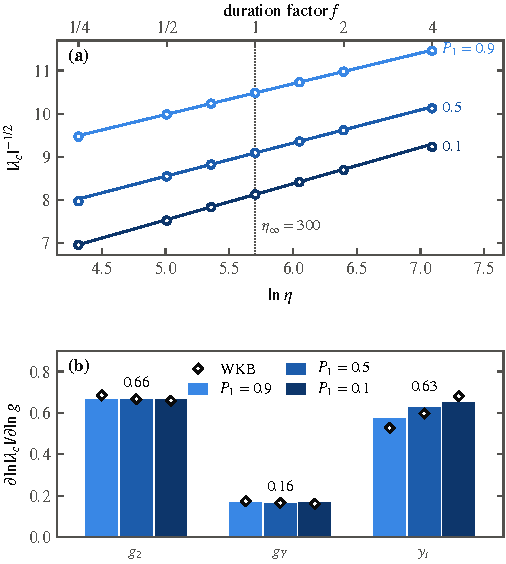
\includegraphics[width=0.7\textwidth]{prd_universality}
\caption{Universality of the finite-volume threshold.
(a)~$|\lamc|^{-1/2}$ grows linearly with the logarithm of the conformal duration $\eta=f\eta_\infty$ for $\Pone=0.9$, $0.5$, and $0.1$ (circles: hazard thresholds; lines: Eq.~(\ref{eq:rb-eta}) from $f=1$).
(b)~Logarithmic derivatives of $|\lamc|$ with respect to $g_2$, $g_Y$, and $y_t$ at $\mub$ (bars) and their WKB estimates (diamonds): the threshold is set mainly by $g_2$ and $y_t$, nearly independently of $\Pone$.} %
\label{fig:rb-universality}
\end{figure}

\subsection{Other spin structures}
\label{sec:rb-spin}

Tori with one or two periodic edges (spin structures PPA and PAA) also turn around once the holonomy sits at its one-loop vacuum.
On a periodic edge the fermions no longer pin the holonomy: at trivial holonomy the hypercharge curvature on that edge is $\kappa_Y=-1.675$ (PPA) and $-1.029$ (PAA), against $+0.700$ for AAA. %
Scanning the hypercharge, SU(2) Cartan, and SU(3) center holonomies edge by edge, we find that the one-loop vacuum on each periodic edge is an SU(3) center element, under which the quarks are twisted by $\pm\frac13$ and the Higgs, $W$, $B$, and gluons are not twisted; it lies $7.89/L$ (PPA) and $4.69/L$ (PAA) below the trivial holonomy per edge. %
This raises the Casimir weight to $\NC=21.07$ (PPA) and $23.67$ (PAA), compared with $25.52$ for AAA, and the shape has a tetragonal stationary point, at which $\NC=19.72$ and $22.84$; as for the AAA cube, the energy is a maximum along the aspect directions. %
The backgrounds differ little: $\Lb\MPbar=655$ and $693$, $\eta_\infty=331$ and $312$, and $\mub=3.72\times10^{15}$ and $3.51\times10^{15}\GeV$, which by themselves move $m_c$ by $-0.03$ and $-0.01\GeV$. %

The Higgs zero mode exists in both cases, because the Higgs is not twisted, and there are no fermion zero modes, because Grassmann constant modes require three periodic edges.
Two ingredients of the zero-mode model change.
The top-quark tadpole, $\propto Z_1(\vartheta_{\rm top})$, is $0.851$ (PPA) and $0.933$ (PAA) times its AAA value. %
The hypercharge curvature on the periodic edges stays negative at the center vacuum, $\kappa_Y=-0.556$ and $-0.304$, so the $\bm w$ direction is inverted, $\Omega_{\rm eff}^2(r)+\Omega_{X,i}^2<0$, for $r<1.5$ (PPA) and $r<1.1$ (PAA), across the well of the resonance. %
Our isotropic $(r,|\bm w|)$ model with a quadratic $\Omega_X^2$ does not apply there; it would need the exact twist energy along the periodic edges, an anisotropic $\bm w$, and the top matching at center holonomy.
An indicative estimate, which scales the cross terms with the direction-averaged curvatures and adds the changes of the background and of the top-quark tadpole, gives $\Delta m_c\approx+0.08$ and $+0.02\GeV$ relative to AAA, or $|\Delta\lamc|\lesssim0.0013$: the magnitude of $\lamc$ is unchanged, and its exact value depends on the sector and needs an anisotropic model. %
At trivial holonomy the fully periodic torus has $\NC=-30$ and does not turn around; with an SU(3) center holonomy its weight is positive, $\NC=11.2$, but the cusps of the lepton zero modes destabilize the electroweak holonomy, and we do not analyze this sector. %

\subsection{Sectors with 't~Hooft flux}
\label{sec:rb-flux}

Requiring all Standard Model fields to be single valued in a twisted sector, the $Z_6$ structure of the Standard Model allows a non-trivial SU(3) or SU(2) twist only together with a hypercharge flux, and the minimal flux is $|\Phi_Y|=2\pi$, reached for $(k_3,k_2)=(\pm1,1)$; a twist in SU(3) alone needs $4\pi$, and in SU(2) alone $6\pi$. %
The classical energy of the flux is
\begin{equation}
E_{\rm flux}=\frac{\Phi_Y^2}{2g_Y^2L}\ge\frac{2\pi^2}{g_Y^2L}=\frac{100.7}{L}, %
\label{eq:rb-flux}
\end{equation}
which is $2.36$ times the entire AAA Casimir energy; a turn would need $\NC>60$, whereas the Standard Model content gives at most $25.5$ in any flat twist, so these sectors cannot turn around. %
In them the Higgs doublet has no constant mode; its lowest mode is a Landau level with $\omega_0=\sqrt\pi/L$, and Landau levels replace zero-point confinement.
The corresponding threshold is $\lamc\approx-1$ ($-0.97$, $-1.36$, and $-1.84$ at $\Pone=0.9$, $0.5$, and $0.1$, uncertain by a factor of about $1.5$ through the Abrikosov parameter), two orders of magnitude more negative than for AAA, but irrelevant for the criterion because these sectors host no turn. %
The threshold of about $-0.01$ is therefore not an accident of the discrete choice AAA, while its precise value, to $10$--$20\%$, depends on the sector and on the Standard Model inputs. %

\subsection{The curvature coupling: zero-mode condition}
\label{sec:rb-xic}

The survival probability $\Pone$ applies when the late turn does not destroy the zero mode, which sets a lower bound on the Higgs curvature coupling $\xiH$.
Under assumption (A6), $\xiH$ is defined at $\mub$ as the coefficient of $R\,\Phi^\dagger\Phi$ in the zero-mode Hamiltonian; it is required by renormalization in curved spacetime~\cite{Birrell:1982ix}, so this is a condition on a Standard Model parameter.
For $\xiH<1/6$ the inverted oscillator of Eq.~(\ref{eq:rb-conformal}) acts, and we follow it with the lens transformation and the quantum--classical switch of Sec.~\ref{sec:rb-late}.
We define the threshold by
\begin{equation}
P_{\rm surv}(\xic)=0.99\,P_{\rm surv}(\tfrac16), %
\label{eq:rb-xic}
\end{equation}
with $P_{\rm surv}$ from the real-time evolution; for $\xiH\ge\xic$ the survival probability is $\Pone$ to $1\%$.
The main uncertainty is the late-time running prescription of $\lambda$ (Sec.~\ref{sec:rb-late}), and we quote the midpoint and half-difference.

\begin{table}[t]
\centering
\caption{Zero-mode threshold $\xic$ on $\xiH(\mub)$ in the final model, with the half difference of the two running prescriptions, the range over all prescription and switching variants, and the electroweak-scale image $\xi_{\rm EW}$.} %
\label{tab:rb-xic}
\begin{tabular}{ccccc}
\toprule
$m_t$ [GeV] & $\Pone$ & $\xic(\mub)$ & Range & $\xi_{\rm EW}$ \\
\midrule
$172.2$ & $0.985$ & $0.0346(40)$ & $0.030$--$0.039$ & $0.0525$ \\ %
$172.6$ & $0.843$ & $0.0737(25)$ & $0.071$--$0.077$ & $0.0862$ \\ %
$172.95$ & $0.511$ & $0.1195(6)$ & $0.119$--$0.121$ & $0.1258$ \\ %
$172.96$ & $0.499$ & $0.1206(7)$ & $0.120$--$0.121$ & $0.1267$ \\ %
$173.0$ & $0.455$ & $0.1248(5)$ & $0.124$--$0.126$ & $0.1304$ \\ %
\bottomrule
\end{tabular}
\end{table}

Table~\ref{tab:rb-xic} gives the threshold in the final model. %
We obtained it by repeating the whole real-time chain with the final cross terms: $145$ node potentials, a calibration that converged to $|\Delta\ln\Gamma|\le6\times10^{-8}$ with $A=0.0124$--$0.0144$, and $55$ real-time evolutions; with the earlier cross terms the same chain reproduces the earlier node potentials exactly. %
At the measured top mass the survival probability stays within $1\%$ of its conformal value for $\xiH(\mub)\gtrsim\xiHcentral$, or $\gtrsim\xiHmin$ including all prescription variants, and at the $\Pone=1/2$ point, $m_t=172.9595\GeV$, interpolation gives $\xic=0.1205(7)$, that is $\xiH\gtrsim\xiHhalf$. %
Below the threshold the survival probability decreases gradually: at $m_t=172.6\GeV$ it falls by $3.5$--$5\%$ at $\xiH=0.04$ and by $13$--$19\%$ at $\xiH=0.02$, and only for $\xiH\to0$ does the zero mode run away (Sec.~\ref{sec:rb-late}). %
The two-dimensional real-time evolution agrees with the calibrated one-dimensional model to $2\times10^{-4}$ in $P_{\rm surv}$ and to $1.4\times10^{-4}$ in $\xic$. %

\paragraph{Universality of $\xic(\Pone)$.}
The threshold is close to a universal function of $\Pone$.
Two versions of the model and the 11 of the 16 variants of the Standard Model inputs and $\alpha_s$ whose $\Pone$ lies in the tested range $0.45\lesssim\Pone\lesssim0.998$ lie on one curve $\xic(\Pone)$ to within $0.002$, and the final model lies on it to $0.0002$ [Fig.~\ref{fig:rb-hazard}(c)]. %
At fixed $m_t$ the final corrections lower $\xic$ by $0.0004$, because they raise $\Pone$. %
Stated through $\Pone$, or through $\lambda(\mub)$, the condition is therefore free of the Standard Model and $\alpha_s$ errors at first order.
At fixed $m_t=172.6\GeV$ these errors widen $\xic$ by $\pm\xiHbandSM$ and $\pm\xiHbandAs$, respectively. %
These bands were computed with the earlier model by shifting $\lambda$ by $\mp|d\lambda(\mub)/dm_t|\times0.10\GeV$ and by repeating the chain at $\alpha_s=0.1171$ and $0.1189$; through the universal curve they carry over to the final model with their midpoints lowered by about $0.0004$. %
In the earlier model they are $0.0750\pm0.0130$ and $0.0795\pm0.0397$ at $m_t=172.6\GeV$ (midpoint and half width). %
The two sides are asymmetric because $\xic$ saturates toward $1/6$ as $\Pone\to0.1$.
The scale of $\xiH$ adds a smaller ambiguity: the $\xiH$-dependent loss occurs at $\tau\approx3.5$--$6$, where $\mu\approx10^{13}$--$10^{14}\GeV$, and the running of $\xi$ between there and $\mub$ is estimated at $0.0005$--$0.002$. %

\paragraph{Running to the electroweak scale.}
The coupling runs as~\cite{Herranen:2014cua,Mantziris:2020rzh}
\begin{equation}
\xi(\mu)=\tfrac16+\bigl(\xi_{\rm EW}-\tfrac16\bigr)\Xi(\mu),\qquad
16\pi^2\frac{d\ln\Xi}{d\ln\mu}=12\lambda+6y_t^2-\tfrac32g_Y^2-\tfrac92g_2^2,
\label{eq:rb-xirun}
\end{equation}
with $\Xi(\mub)=1.155$, so that $\xiH(\mub)=\xiHmin$ corresponds to $\xi_{\rm EW}\approx\xiHminEW$ at $\mu=m_t$; the conformal value $1/6$ is a fixed point of the one-loop running. %

\subsection{The curvature coupling: all-mode bound during inflation}
\label{sec:rb-xiinf}

After the turn the plateau inflates, and long-wavelength Higgs fluctuations can nucleate the true vacuum~\cite{Espinosa:2007qp,Hook:2014uia,Kearney:2015vba,Espinosa:2015qea,Joti:2017fwe,Markkanen:2018pdo}.
The plateau of assumption (A3) is a minimally coupled scalar with a Starobinsky-shaped potential and no $R^2$ term, so the field-theory criterion of Ref.~\cite{Mantziris:2020rzh} applies, and the $R^2$ bound $\xi_{\rm EW}\gtrsim0.1$ of Ref.~\cite{Mantziris:2022fuu} does not. %
We use the one-loop curved-space effective potential of Ref.~\cite{Markkanen:2018bfx} with renormalization-group improvement,
\begin{equation}
V_{\rm RGI}=\tfrac12\xi(\mu_*)Rh^2+\tfrac14\lambda(\mu_*)h^4+\frac{\alpha(\mu_*)}{144}R^2,
\label{eq:rb-VRGI}
\end{equation}
where $h$ is here the Higgs field, $\mu_*$ the field- and curvature-dependent renormalization scale, and $\alpha$ the coefficient of $R^2$ generated by the running, together with the Hawking--Moss rate~\cite{Hawking:1981fz}
\begin{equation}
\Gamma_{\rm HM}=\Bigl(\frac{R}{12}\Bigr)^2e^{-B},\qquad B=\frac{384\pi^2\Delta V}{R^2},
\label{eq:rb-HM}
\end{equation}
with $\Delta V$ the height of the barrier of $V_{\rm RGI}$.
We require less than one bubble in the past light cone, $\langle N\rangle=\int\gamma(N)\,dN<1$, where
\begin{equation}
\gamma(N)=\frac{4\pi}{3}\Bigl[a_{\rm inf}\Bigl(\frac{3.21\,e^{-N}}{H_0}-\tilde\eta\Bigr)\Bigr]^3\frac{\Gamma_{\rm HM}}{H},\qquad \frac{d\tilde\eta}{dN}=-\tilde\eta-\frac{1}{a_{\rm inf}H},\quad\tilde\eta(0)=0,
\label{eq:rb-lightcone}
\end{equation}
counts the bubbles per $e$-fold $N$ of inflation in the past light cone of today's observer, following Refs.~\cite{Mantziris:2020rzh,Mantziris:2022fuu}, with the background integrated without the slow-roll approximation. %
The end of inflation is $\dot H/H^2=-\frac14$; taking $\ddot a=0$ instead changes the bound by less than $10^{-4}$, and the start of the integration at the turn ($N=68.47$) does not matter, because the integral is dominated by the last $e$-folds. %
On the torus the past light cone is cut by the cube of edge $6/H_0$, which keeps $98.1\%$ of its volume ($\Delta B=0.019$), a negligible change. %
This implementation reproduces $\xi_{\rm EW}=0.05946$ of Ref.~\cite{Mantziris:2020rzh} (target $0.05938$). %

For $m_t=172.2$, $172.6$, and $173.0\GeV$ we find $\xi_{\rm inf}(\mub)=0.030$, $0.038$, and $0.044$, or $\xi_{\rm EW}=0.049$, $0.055$, and $0.060$. %
At the same scale the zero-mode threshold and the inflationary bound coincide at $\lambda(\mub)\approx-0.0065$, i.e., $m_t\approx172.1\GeV$, and the zero-mode condition is the stronger one above this mass (Fig.~\ref{fig:rb-xi}). %
The two calculations cover adjacent epochs: the zero-mode calculation until the torus leaves the Hubble radius about five $e$-folds after the turn, and the light-cone count afterward; the transition contributes at most $O(10)\,e^{-B}$ with $B\gtrsim180$ to $\langle N\rangle$, but we have not simulated it jointly. %

After inflation the plateau oscillates with $H_{\rm end}\approx7\times10^{12}\GeV$, far above the instability scale, so the analysis of Ref.~\cite{Herranen:2015ima} applies: $\xi\lesssim1$ avoids destabilization by curvature oscillations, and $\xi<3/8$ avoids tachyonic resonance. %
The allowed window is
\begin{equation}
\max(\xic,\xi_{\rm inf})\le\xiH\lesssim1,
\label{eq:rb-window}
\end{equation}
and the conformal value $\xiH=1/6$ lies inside it in both scale readings.

\begin{figure}[t]
\centering
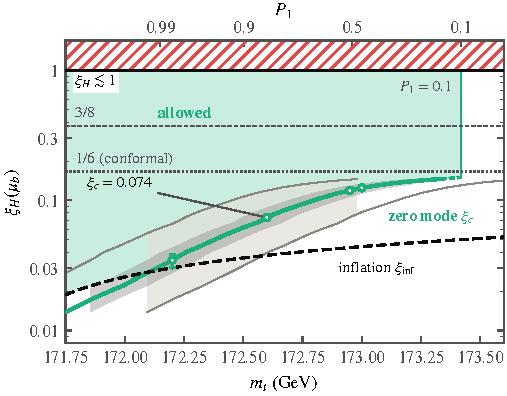
\includegraphics[width=0.6\textwidth]{prl_fig3_xi}
\caption{Curvature coupling needed for survival.
The zero-mode threshold $\xic(\mub)$ (solid; circles: direct calculations; dark and light bands: Standard Model mapping and $\alpha_s$) and the all-mode bound $\xi_{\rm inf}$ from plateau inflation (dashed) bound $\xiH$ from below, and $\xiH\lesssim1$~\cite{Herranen:2015ima} bounds it from above (hatched).
Survival with $\Pone\geq0.1$ requires $\xiH$ in the shaded region; the dashed end of the line extrapolates below $\Pone=0.13$.
Dotted: the conformal value $1/6$; thin dashed: $\xi=3/8$.
The zero-mode condition is the stronger one for $m_t\gtrsim172.1\GeV$.} %
\label{fig:rb-xi}
\end{figure}
